\documentclass[main.tex]{subfiles}
\begin{document}

\section{Sheet 9}

\subsection{Censorship principle justification}

\subsubsection{Boundary condition}

We assume that the Kerr black hole starts off as \emph{critical}: so initially we have \(a = GM\), and that the particle's addition makes it so that \(a' \geq G M'\): this can be written by making the dependence on \(J = aM\) explicit: when we add the particle we get \(J'= J + lm\) and \(M' = M + me\). So the condition reads: 
%
\begin{subequations}
\begin{align}
  J' &\geq G M^{\prime 2}  \\
  J + lm &\geq G \qty(M^2 + 2mMe + (me)^2)  \\
  l &\gtrsim 2GM e
  \,,
\end{align}
\end{subequations}
%
where we used the fact that \(J = G M^2\) and we ignored the \(O(m^2)\) term, which is negligible. 
Hereafter, we assume that we have exactly the boundary condition \(l = 2GMe\). 

\subsubsection{Effective potential barrier}

We write the potential with respect to the adimensional coordinates \(R = r/2GM\) and \(L= l/2GM = e\), and we  use the fact that \(a = GM\), which implies \(a/2GM = 1/2\). With these substitutions, we find: 
%
\begin{align}
  V _{\text{eff}} (R, e, L) &= 
  - \frac{1}{2R} 
  + \frac{L^2 -  (e^2 - 1) / 4 }{2R^2}
  - \frac{(L - e/2)^2}{2R^3}  \\
  &=   - \frac{1}{2R} 
  + \frac{e^2 -  (e^2 - 1) / 4 }{2R^2}
  - \frac{e^2}{8R^3}  \\
  &= e^2 \qty(\frac{3}{8R^2} - \frac{1}{8R^3}) - \frac{1}{2R} + \frac{1}{8R^2}
\,.
\end{align}

We want to see, then, whether the potential barrier is as high as \((e^2- 1) /2\). Where is this potential barrier? 
The photon is absorbed when it gets inside the event horizon (which then should disappear), and we know that the locations of the horizons are given by \(r_{\pm} = GM \pm \sqrt{(GM)^2 - a^2} = GM\), so in our case they are situated at \(R = 1/2\). 

Plugging this into the formula we find 
%
\begin{align}
  V _{\text{eff}} = e^2 \qty(\frac{3}{2} - 1) - 1 + \frac{1}{2} = \frac{e^2 -1}{2}
\,,
\end{align}
%
so at \(R = 1/2\) we must have \(\dv*{r}{\tau } = 0\).
This is actually enough for our purposes, but it is interesting to see the global shape of the effective potential, so I made a plot of it. 

\begin{figure}[ht]
  \centering
  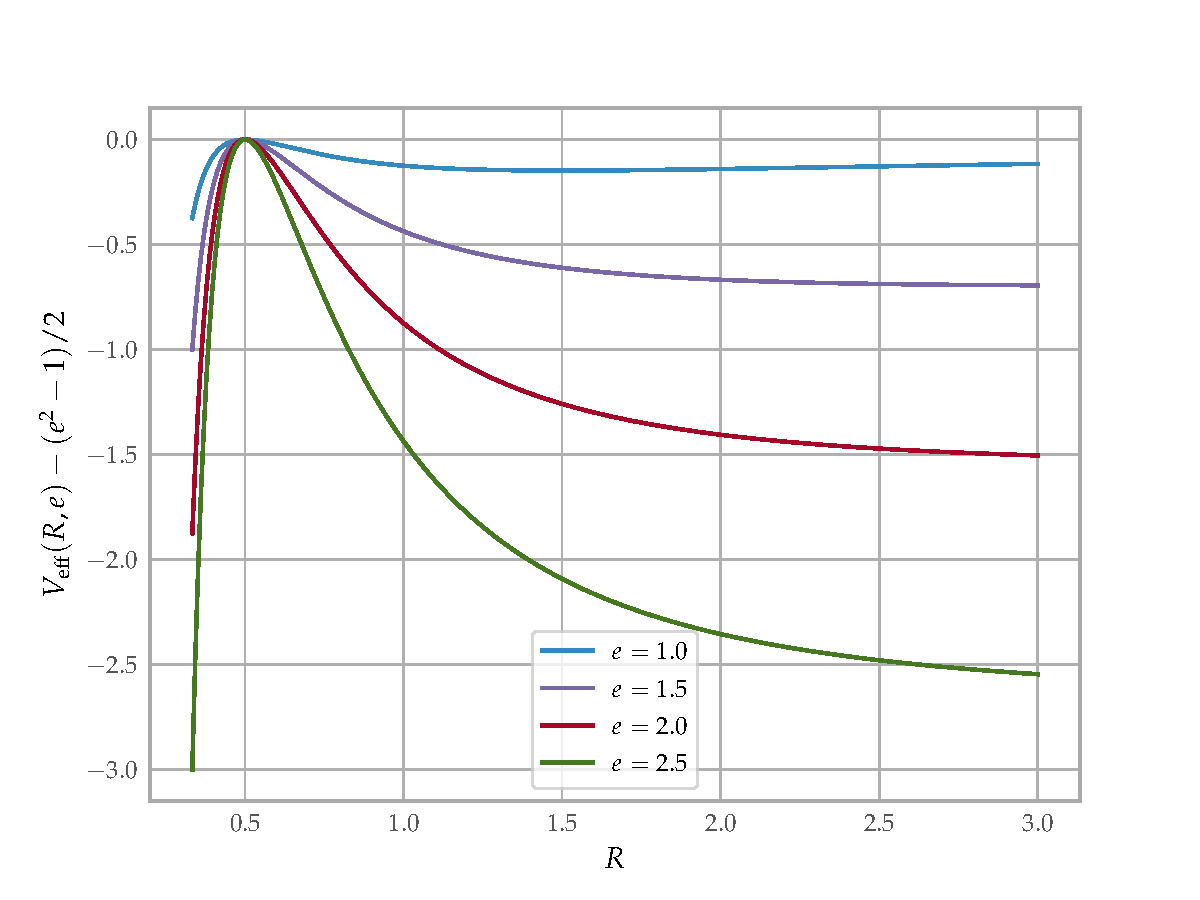
\includegraphics[width=\textwidth]{figures/potential_barrier}
  \caption{Effective potential \(V _{\text{eff}} (R, e) - (e^2 -1) / 2\).}
  \label{fig:residual-potential}
\end{figure}

\subsubsection{Comments on the possibility of undressing a singularity (complement)}

We have shown that the potential barrier will prevent a particle with angular momentum \(l\) with respect to the BH from being absorbed. 
There are some things to consider: one of these is the fact that we assumed \(m^2\) is negligible: what if we threw a \emph{really massive} object into our Kerr black hole?
In that case we would have \(L = e + m e^2 / 2M > e\), and since \(\dv*{V}{L} > 0\) everywhere the potential barrier would be even higher. This is not the way to go. 

However, we neglected \emph{intrinsic} spin: what if we threw lots of, say, electrons aligned with the rotation axis down on the BH? 
They may have angular momentum with respect to the hole which allows them to go in, but increase its angular momentum by a little bit more through their intrinsic spin in order to make the singularity naked\dots

\subsection{Kerr geometry null surfaces}

\subsubsection{Horizon metric}

Let us compute the metric elements at the outer horizon: it is a straight calculation. We just substitute in \(r = r_{+} = GM + \sqrt{(GM)^2 - a^2}\) and \(\rho^2 = \rho^2_{+}\): 
%
\begin{subequations}
\begin{align}
  &g_{00}  = - \qty(1 - \frac{2GMr_{+}}{\rho_{+}^2})  \\
  &= \frac{1}{\rho_{+}^2} \qty(2GM \qty(GM + \sqrt{(GM)^2 - a^2}) - r_{+}^2 - a^2 \cos^2\theta )  \\
  &= \frac{1}{\rho_{+}^2} \qty( 2 (GM)^2 + 2GM \sqrt{\dots}- \qty((GM)^2 + (GM)^2 -a^2 + 2GM \sqrt{\dots}) - a^2 \cos^2 \theta )  \\
  &= \frac{a^2}{\rho_{+}^2}  \qty(1 - \cos^2 \theta ) = \frac{a^2 \sin^2\theta}{\rho_{+}^2}
\,,
\end{align}
\end{subequations}
%
where we omitted the argument of the square root for brevity: it is the same on either side, and it simplifies. 
For the components \(g_{03}\) and \(g_{22} \) we cannot simplify anything. The  only thing to recall is that the off-diagonal components of the metric when written in component form are half of what they are when written with respect to the differentials, since we usually do not bother to write two separate \(\dd{t} \dd{\varphi }\) and \(\dd{\varphi } \dd{t}\) terms: the diffentials commute, therefore we simply write one of the two combinations with double the value. So we have: 
%
\begin{align}
  g_{03} = -\frac{2GMa r_+ \sin^2\theta }{\rho_{+}^2}
\,
\end{align}
and 
%
\begin{align}
  g_{22} = \rho_{+}^2
\,.
\end{align}

The computation of the \(g_{33} \) component\footnote{There is a typo in the assignment: this component is denoted as \(g_{03}\) again.} is more interesting: we get 
%
\begin{align}
  g_{33} = \qty( r_+^2 + a^2 + \frac{2GMr_{+} a^2 \sin^2\theta }{\rho_{+}^2}) \sin^2 \theta 
\,,
\end{align}
%
and we recall the definition of \(\Delta = r^2 + a^2 - 2GM r\): since we are dealing with the case in which \(\Delta = 0\), so we have \(r^2 + a^2 = 2GMr\), which we substitute in and collect:
%
\begin{align}
  g_{33} &= 2GMr_{+} \qty(1 + \frac{a^2 \sin^2\theta }{\rho_{+}^2}) \sin^2\theta \\
  &= 2GMr_{+} \frac{\sin^2 \theta }{\rho_{+}^2} \qty(r_{+}^2 + a^2 \cos^2 \theta + a^2 \sin^2\theta )
\,,
\end{align}
%
and then we can notice again the combination \(r_{+}^2 + a^2 = 2GMr_{+}\): so in the end we get 
%
\begin{align}
  g_{33} = \qty(\frac{2GMr_{+} \sin \theta }{\rho_{+}})^2
\,.
\end{align}

\subsubsection{Uniqueness of the null vector}

The metric we found for the 3D space \(r \equiv r_{+}\) is: 
%
\begin{align}
  \dd{s^2} = \frac{a^2 \sin^2\theta }{\rho_{+}^2} \dd{t^2} 
  - \frac{4GM a r_{+} \sin^2\theta }{\rho_{+}^2} \dd{t} \dd{\varphi } + \rho_{+}^2 \dd{\theta^2}
  + \qty(\frac{2GMr_{+} \sin \theta }{\rho_{+}})^2 \dd{\varphi^2}
\,,
\end{align}
%
and now we want to find a vector field \(l^{\mu } = (l^{t}, l^{\theta }, l^{\varphi })\) such that \(l^2 = l^{\mu } g_{\mu \nu } l^{\nu } = 0\). 
Since \(\rho_{+}^2 \neq 0\) we can multiply everything by it: we get 
%
\begin{align}
  l^2 = a^2 \sin^2\theta (l^{t})^2 
  - 4GMar_{+} \sin^2\theta l^{t} l^{\varphi }
  + \rho_{+}^{4} (l^{\theta })^2
  + (2GMr_{+})^2 \sin^2 \theta (l^{\varphi })^2
\,,
\end{align}
%
and we notice that the \(tt\), \(\varphi \varphi \) and \(\varphi t\) terms form a square: we find 
%
\begin{align}
  l^2= \qty(a \sin \theta l^{t} - 2GMr_{+} \sin \theta l^{\varphi })^2 + \rho_{+}^4 (l^{\theta })^2
\,,
\end{align}
%
so if we want to set \(l^2 = 0\) we need to have both square terms be separately equal to zero. 
This means that \(l^{\theta } = 0\), and that 
%
\begin{align}
  a l^{t} = 2GMr_{+} l^{\varphi }
\,,
\end{align}
%
so if we choose a value for one of the components the other one is fixed. Therefore, the vector field only has a scalar degree of freedom: we can rescale it by a scalar field, but its direction is fixed. Specifically, we find that 
%
\begin{align}
  \frac{l^{\varphi }}{l^{t}}  = \frac{a}{2GMr_{+}}
\,
\end{align}
%
is the only allowed ratio of these components. If we interpret the vector \(l\) as the 4-velocity of light trapped at the horizon, we have 
%
\begin{align}
    \dv{\varphi }{\tau } \dv{\tau }{t} = \dv{\varphi }{t}
    = \frac{a}{2GMr_{+}}
\,.
\end{align}

\subsubsection{A basis for the horizon}

The \(\varphi \varphi \) and \(\theta \theta \) components of the metric are squares of real numbers, so they are positive, so the vectors \(m^{\alpha } = [0,0,1,0]^{\top}\) and \(n^{\alpha } = [0,0,0,1]^{\top}\) are spacelike. 

They are orthogonal, since \(m^{\alpha } g_{\alpha \beta } n^{\beta } = g_{23} =0 \). 
Let us compare them to the null vector we found earlier, for which we can use the normalization: \(l^{\alpha } = [2GMr_{+}, 0, 0, a]^{\top}\). 
We have that \(m^{\alpha } g_{\alpha \beta } l^{\beta } = g_{2 \beta } l^{\beta }=  0\), since the only \(2 \beta \) component of the metric is \(g_{22 }\) but \(l^{2}=0\). On the other hand, we have 
%
\begin{align}
  n^{\alpha }g_{\alpha \beta } l^{\beta } 
  &= g_{3 \beta } l^{\beta } \\
  &= -\frac{ 2GMar_{+}\sin^2\theta }{\rho_{+}^2} 2GMr_{+}
  + \qty(\frac{2GMr_{+} \sin \theta }{\rho_{+}})^2 a = 0
\,.
\end{align}

A basis is defined by linear independence and spanning, which are properties independent of the metric. For an \(n\)-dimensional set of vectors, each of these properties is equivalent to our set being a basis.

So, we prove linear independence: let us consider a combination of these vectors: 
%
\begin{align}
  A l^{\mu } + B m^{\mu } + C n^{\mu } = 0
\,,
\end{align}
%
and we need to show that this implies \(A = B = C = 0\). 
In order for the \(\mu = 0\) component of the result to be zero we need \(A = 0\). In order for the \(\mu =2\) component to be zero we need \(B = 0\). In order for the \(\mu = 3\) component to be zero we need \(C = 0\), so the result is proven. 

\subsection{Solar system Kerr}

\subsubsection{Earth's implausible Kerr description}

We need to estimate the angular momentum of the Earth: for our order of magnitude calculation we will model it as a constant-density sphere, with \(M = \SI{6e+24}{kg}\) and \(r = \SI{6e6}{m}\). The moment of inertia is then given by 
%
\begin{align}
  I = \frac{2}{5} M r^{2} \approx \SI{1e38}{kg m^2}
\,.
\end{align}

This is a slight over-estimate: more of the Earth's mass is concentrated around the center, so the actual moment of inertia is about \(20\%\) lower. This is close enough for our purposes. 

Then, since the Earth rotates at a revolution per day so with \(\omega = 2\pi / \SI{1}{d}\), we have our estimate for the angular momentum: 
%
\begin{align}
  J = I \omega 
  \approx \SI{7e+33}{kg m^2 s^{-1}}
\,.
\end{align}

In order to find the length corresponding to the natural-units formula \(a = J/M\) we need to divide by \(c\): so we get 
%
\begin{align}
  a = \frac{J}{Mc} \approx \SI{4}{m}
\,,
\end{align}
%
while we have \(GM/c^2 \approx \SI{4e-3}{m}\): their ratio is of the order \num{e3}.

This of course does not mean that there is a naked singularity deep inside the Earth: we'd need all the mass to be concentrated around \(r=0\) for that to be the case, and instead the radius of the Earth is quite larger than \SI{4}{m}.

So we have the quite interesting result that the general-relativistic description of the Earth corresponds to a Kerr metric with \(a \gg GM\). It is not really clear to me what meaning should be drawn from this but it seems to be the case. 

\subsubsection{The Sun's Kerr metric}

We can do the same calculation for the Sun, which has \(m \approx \SI{2e30}{kg}\) and \(r \approx \SI{7e8}{m}\); its moment of inertia factor (\(I  / Mr^2\)) is quite badly approximated by \(2/5\): it is around \(0.07\).\footnote{\url{https://web.archive.org/web/20191030204430/https://nssdc.gsfc.nasa.gov/planetary/factsheet/sunfact.html}}
The rotation of the Sun depends on the latitude of the surface since it is a fluid, but its period is on the order of \(\SI{600}{hr}\). 
So we have 
%
\begin{align}
  J = I \omega \approx \SI{1.7e41}{kg m^2 s^{-1}}
\,,
\end{align}
%
which gives 
%
\begin{align}
  a = \frac{JM}{c} \approx \SI{330}{m}
\,,
\end{align}
%
while 
%
\begin{align}
  \frac{GM}{c^2} \approx \SI{1500}{m}
\,,
\end{align}
%
therefore the ratio \(a/GM\) is around \num{0.2}. 
So the Sun's Kerr metric would have an inner and outer horizon. 

\subsubsection{Critical \(\omega \) in general (complement)}

We can compute the value of \(\omega \) for which any object will have \(a = GM\): if the moment of inertia is \(I = \kappa M r^2\) in the end we find 
%
\begin{align}
  \omega _{\text{crit}} = \frac{GM}{\kappa r^2 c}
\,,
\end{align}
%
so if we consider objects with a constant density \(\rho \sim M r^{-3}\) the critical angular velocity scales with \(r\): it gets quite low for small objects! 
A carousel with \(r \sim \SI{2}{m}\) and \(M \sim \SI{100}{kg}\) (and \(\kappa \sim 0.5\)) will have a critical angular velocity of around \SI{e-17}{rad/s}! It is \emph{really easy} for a small object to have \(a \gg GM\). 

\end{document}